\chapter{Physics-Informed Neural Networks}\label{ch:pinns}

Although the idea of incorporating prior knowledge in a neural network for solving a PDE is not new~\cite{dissanayake1994}, we can consider the first Physics-Informed Neural Networks (PINNs) to have been introduced in 2017 in a two-part article~\cite{raissi_physics_2017,raissi_physics_2017-1}, which later merged into a single paper~\cite{raissi_physics-informed_2019}. PINNs are Neural Networks (NN) that encode the equations of physical models, including PDEs, as a component of the network itself. PINNs approximate the solutions of PDEs using a neural network, trained by minimizing a loss function. The specificity of PINNs lies in this loss function, which typically takes the form of a physical equation and also includes boundary conditions. This loss function is the key difference between PINNs and classical neural networks, which try to adjust their weights to best fit the data presented during training.
\par The PINN method is thus a meshless solution technique, finding the solutions to a PDE not by solving a governing equation, but by minimizing a certain loss function. This particular loss function restricts the space of acceptable solutions, thereby enabling the problem to be solved with satisfying accuracy.

\section{Definition}

One of the advantage of PINNs over typical neural networks is their ability to solve problems with very little, or noisy data. Due to their structure, PINNs are used to solve differential equations, which in their most general form can be written as~\cite{cuomo_scientific_2022}:

\begin{equation}
    \label{eq:pde-general}
    \begin{split}
        \mathcal{F}\left[ u(z); \lambda \right] &= f(z) \text{, } z \in \Omega\\
        \mathcal{B}\left[ u(z) \right] &= g(z) \text{, } z \in \partial\Omega
    \end{split}
\end{equation} where $u(z)$ denotes the solution to be determined, $\mathcal{F}[.;\lambda]$ is a non-linear operator parameterized by $\lambda$, $f$ is a function defining the problem data, $\mathcal{B}$ is an operator indicating a boundary, $g$ is a boundary function, and $\Omega$ is a subset of $\mathbb{R}^D$. Here, $z$ denotes the spatio-temporal domain. In our case, the equations are time-independent, and the integration will be carried out only over the spatial domain.

More concretely, the underlying methodology of PINNs can be summarized in three parts. First, the solution $u(z)$ is approximated by a neural network parameterized by a set of parameters $\theta$. Then, for a differential equation of the type
\begin{equation}
\label{eq:pde-exemple}
u_t + \mathcal{F}[u;\lambda] = 0\text{, } x\in \Omega\text{, } t \in [0, T]\text{,}
\end{equation} we set
\begin{equation}
p \coloneqq u_t - \mathcal{F}[u;\lambda] \text{.}
\end{equation} This function $p$ is referred to as a \emph{physics-informed neural network}. Finally, the network learns to approximate the differential equation by finding the set of parameters $\theta$ that minimizes the loss function $\mathcal{L}(\theta)$:

\begin{align}
    \label{eq:PINN-argmin-loss}
    \theta^* &= \underset{\theta}{\mathrm{argmin }} \text{ }\mathcal{L}(\theta) \nonumber \\
     &= \underset{\theta}{\mathrm{argmin }} \left( \omega_{\mathcal{F}}\mathcal{L}_{\mathcal{F}}(\theta) + \omega_{\mathcal{B}}\mathcal{L}_{\mathcal{B}}(\theta) + \omega_{data}\mathcal{L}_{data}(\theta) \right)\text{ ,}
\end{align}
where the $\omega_i \text{, } i \in \{\mathcal{F}, \mathcal{B}, \mathrm{data}\}$  are weights for the specific losses $\L_i$, respectively defined for the PDE residual, the boundary and the data. Their expressions are detailed in the following section.

\section{Properties}

\subsubsection{Loss Function}
We note that unlike a typical loss function, we have for the PINNs a weighted sum of several loss functions, each corresponding to one of the training contributions mentioned above; the governing equation residual, the boundary conditions, and the data points.

We first focus on the loss function arising from the difference between the network's prediction and the governing differential equation $\mathcal{F}$ :
\begin{equation}
    \label{eq:pde-loss}
    \mathcal{L}_{\mathcal{F}}(\theta) = MSE_{\mathcal{F}} = \dfrac{1}{N_c}\sum^{N_c}_{i=1} \left\|\mathcal{F}(\hat{u}_{\theta}(z_i)) - f(z_i)\right\|^2
\end{equation} where $N_c$ is the number of points where the PDE residual is evaluated in the domain. These points are called \emph{collocation points}. MSE is the commonly used mean square error. This loss function is computed by taking advantage of the auto-differentiation properties of neural networks (see Section~\ref{sec:AD}) to compute the partial derivatives of $\hat{u}_{\theta}(z)$. Similarly, we then have the error coming from the boundary conditions:

\begin{equation}
    \label{eq:boundary-loss}
    \mathcal{L}_{\mathcal{B}}(\theta) = MSE_{\mathcal{B}} = \dfrac{1}{N_B}\sum^{N_B}_{i=1} \left\|\mathcal{B}(\hat{u}_{\theta}(z_i)) - g(z_i)\right\|^2
\end{equation} where $N_B$ is naturally the number of points used to represent the boundary conditions. Finally, the error due to discrepancies with the data points takes the following form:

\begin{equation}
    \label{eq:data-loss}
    \mathcal{L}_{data}(\theta) = MSE_{data} = \dfrac{1}{N_d}\sum^{N_d}_{i=1} \left\|\hat{u}_{\theta}(z_i)) - u^{*}_i\right\|^2
\end{equation} where $N_d$ is the number of data points. Depending on the problem setup, one can choose higher or lower values for the weights $\omega_i \text{, } i \in \{\mathcal{F}, \mathcal{B}, \mathrm{data}\}$, always with $|\omega_i| \leq 1$. For example, one can decrease the value of $\omega_{\mathcal{F}}$ if the model's PDE is deemed unreliable to describe the system. Or decrease $\omega_{data}$ if the data are noisy. In an inverse problem, PINNs can be used to model the data, while simultaneously solving the PDE. In other words, in an inverse problem a PINN can determine the parameters $\lambda$ from Equation~\eqref{eq:pde-exemple} given some simulation data. Lastly, it is worth noting that in the case of a forward problem, the error related to the data can also represent the boundary conditions. In our case, we will indeed rather use the error $\mathcal{L}_{data}(\theta)$ estimated at the borders, than a loss function as given by equation~\eqref{eq:boundary-loss}. We will then write our loss function as follows:

\begin{equation}
    \label{eq:loss-galaxy}
    \mathcal{L}(\theta) = \dfrac{1}{N_c}\sum^{N_c}_{i=1} \left\|\nabla^2 \hat{\Phi}(z_i) - 4 \pi G \rho(z_i) \right\|^2 + \dfrac{1}{N_B}\sum^{N_B}_{i=1} \left\|\hat{\Phi}(z_i) - \Phi_i \right\|^2
\end{equation}
where $\hat{\Phi}(z_i)$ is the predicted gravitational potential at point $z_i$, and $\Phi_i$ is the real value of the potential at that same point. The procedure described above is summarized in Figure~\ref{fig:loss-pinn}.

\begin{figure}[ht]
    \centering
    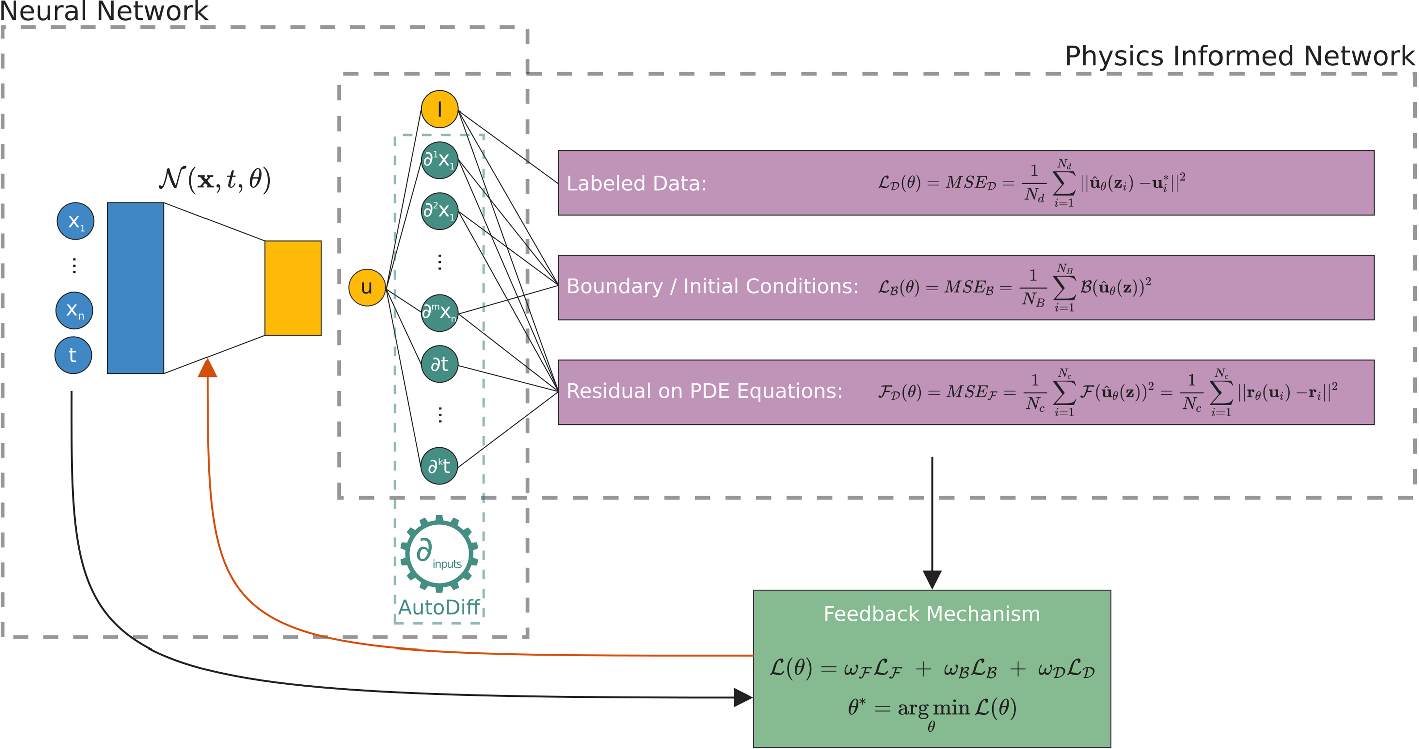
\includegraphics[scale=0.25]{imgs/training-pinn-schema.png}
    \caption{Structure and training procedure of a PINN. The fundamental difference with a typical neural network is the inclusion of a differential equation and boundary terms in the loss function. \textit{Illustration from~\cite{cuomo_scientific_2022}}.}
    \label{fig:loss-pinn}
\end{figure}

\subsubsection{Optimization}

As previously indicated, solving a PDE with a PINN comes down to minimizing the loss function $\mathcal{L}(\theta)$; it's therefore an optimization problem. This process is called \emph{training}. As described in Chapter~\ref{ch:neural-networks}, there are several algorithms to find the minimum of the loss function. However, in most cases~\cite{cuomo_scientific_2022} PINNs are trained using the Adam algorithm, or the Limited-memory Broyden-Fletcher-Goldfarb-Shanno (L-BFGS) method. The Adam approach combines an adaptive learning rate with momentum methods, while the L-BFGS method is a quasi-Newtonian optimization algorithm~\cite{cuomo_scientific_2022}. These two algorithms are predominantly used due to their speed of convergence, compared to a simple gradient descent. Particularly, it is shown in~\cite{he_physics-informed_2020} that in the case where the number of residuals or data points is limited, the L-BFGS-B algorithm\footnote{The L-BFGS-B algorithm extends the L-BFGS algorithm to handle simple box constraints.} is more efficient, with a faster convergence rate and reduced computational cost.

\subsubsection{Activation Function}

As mentioned in chapter~\ref{ch:neural-networks}, there are many possible activation functions to build a model with a neural network. In our case we want our activation function to be at least of class $\mathcal{C}^2$, twice differentiable, since we take the gradient of $\hat{\Phi}(z)$ twice when calculating the Laplacian. Thus, we will mainly use the hyperbolic tangent function in our work, and study the effect of sigmoid, silu or even log-sigmoid functions on the accuracy of our model.

%\subsubsection{Error (optional)}

%We will not detail in this work a formal analysis on the error of PINNs and their limitations. However, this component of the study of PINNs is where the most work remains to be done. Therefore, we wish to provide some theoretical results to support the consistency of our study, but the interested reader can find an exhaustive description of the actual work in this field in~\cite{cuomo_scientific_2022}. In particular, a recent result from~\cite{de_ryck_approximation_2021} proves that the difference $\hat{u} - u$ tends to $0$ when the width of the neural network, with a hyperbolic tangent activation function, tends to infinity. Thus, we ensure that by choosing a neural network, with two hidden layers and a tanh activation function, with a sufficient number of neurons, we will be able to approximate the gravitational potential as closely as desired.

\subsubsection{Architecture}

Since their first implementation in 2017~\cite{raissi_physics_2017} with a Feed-Forward Neural Network (FFNN), PINNs have evolved and transformed. Although the majority of PINNs still use an FFNN architecture, there exist now numerous other implementations with different architectures; convolutional networks, recurrent networks, Bayesian networks, etc. Interested readers can find an exhaustive list of these architectures in the review article~\cite{cuomo_scientific_2022}. For our part, we will use an FFNN, in which each neuron is connected to all the neurons in the next layer, as described in chapter~\ref{ch:neural-networks}. Although the idea of this work is not to strive to find the hyperparameters that provide the optimal results, we will look at the impact that some of these parameters, such as the activation function or the width of the network, have on the accuracy of the PINN.
